\section{Introduction}
\label{sec:Introduction}

Construction industry is becoming increasingly data intensive with the growing use of
information and communication technology in all phases of a building life-cycle. The design phase is
carried out with Building Information Modeling (BIM) tools and systems that produce elaborate
object-oriented 3D models, and the construction phase with a wide range of construction planning,
scheduling, and coordination systems. In the operational stage the building is monitored,
controlled, and maintained based on sensor data and human observations.

In the future, buildings will act as hubs of a wide variety of real-time and historic data about
spaces, indoor locations, indoor routes, assets, people, sensors, materials, equipment, connections
to surrounding networks (traffic, infrastructure, communication), and so on.

A huge amount of design information is already created in the building design phase 
using BIM tools and there is a widely adopted standard, IFC (Industry Foundation Classes) to
represent building designs. IFC has been specified to improve interoperability between different
disciplines in the design phase of a project, including the architecture, structural engineering,
MEP engineering models, and so on. Nowadays, the IFC standard is supported by all the major BIM
vendors; their BIM tools can export building models as IFC files that can be exchanged with other
parties.

The design models can provide the framework with which the information gathered from other sources
can be organized and visualized.  However, despite the IFC standard, the design information is currently
difficult to access and utilize. The sharing of building models based on file exchange does not work
sufficiently well in practice. Utilization of related information from different models requires
repeated manual work from the designers. In the longer run, file exchange cannot provide a fruitful
basis for open utilization of building information and emergence of new, innovative applications.

We have developed a WebIFC converter to derive an OWL ontology from the IFC schema (called ifcOWL),
and RDF datasets from IFC files (called ifcRDF).

The ifcOWL ontology is used to classify concepts, characterize possible relationships, and define possible constraints of data in ifcRDF datasets which replicate the content of original IFC-STEP data files. Thus, all terms defined in the ifcOWL ontology must be based on the corresponding constructs of the original IFC-EXPRESS schema. Ideally, there should be only one ifcOWL ontology for one IFC schema (see Fig. \ref{fig:ifcOWL-single}). However, taking account that ifcRDF datasets are automatically generated, data validation is almost never required. So in most of cases it is wisely to use a lightweight ontology instead of a detailed one in order to facilitate more effective reasoning.

\begin{figure}[h]
\centering
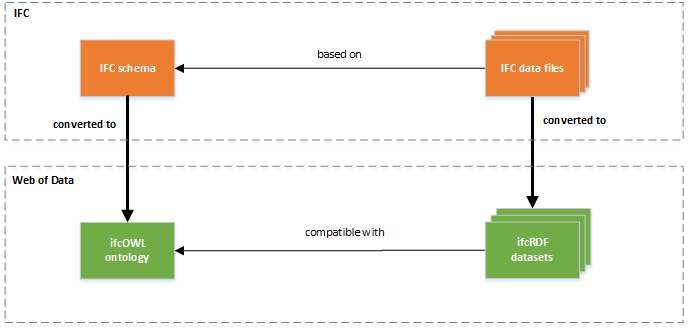
\includegraphics[width=0.75\textwidth]{images/ifcOWL-single.png}
\caption{A single ifcOWL ontology}
\label{fig:ifcOWL-single}
\end{figure}

Various levels of details of ifcOWL ontologies are defined in the Table \ref{tab:ifcOWL-levels}. An ifcOWL ontology version can be considered as extension of all ontology versions with smaller level numbers. 

\begin{table}[h]
\centering
\footnotesize
\begin{tabularx}{\textwidth}{|X|X|X|}
\hline
\textbf{Level (name)} & \textbf{Detail} & \textbf{Note}   \\

\hline
0 (None) & Schema meta data &   \\

\hline
1 & All type names &   \\

\hline
2 & Entity type hierarchy &   \\

\hline
3 & Enumeration \& Select data types & \\

\hline
4 (Lite) & Property names and value types &   \\

\hline
5 & Keys &   \\

\hline
6 (Standard) & Inverse properties &   \\

\hline
7 & Property cardinality restrictions  &   \\

\hline
8 (Advanced) & List type cardinality restrictions  &   \\

\hline
9 (Full) & Property value types with exact value ranges  & Not supported by the converter  \\

\hline
\end{tabularx}
\caption{Levels of details of ifcOWL ontology}
\label{tab:ifcOWL-levels}
\end{table}

Having multiple versions of the same ontology and knowing exactly that every ifcRDF dataset will be compatible with any related ifcOWL ontology (see Fig. \ref{fig:ifcOWL-multilayered}) user can choose the best one based on the requirements of the concrete use case and tools used. For instance, when it is required to query entity properties, extract the type hierarchy, or convert ifcRDF datasets back to object-oriented data models it is enough to use \textbf{ifcOWL-Lite} ontology. It case of reasoning about data including inverse properties, it is recommended to use \textbf{ifcOWL-Standard} ontology. When data validation, for example, checking type and cardinality constraints is needed \textbf{ifcOWL-Advanced} ontology is the most reasonable choice.

\begin{figure}[h]
\centering
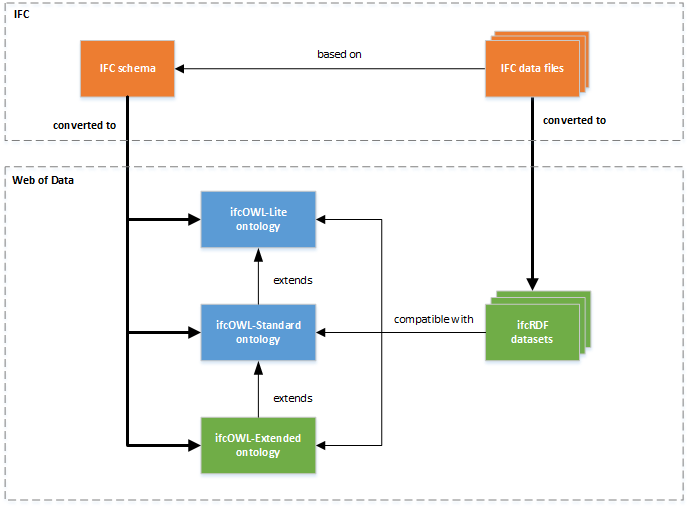
\includegraphics[width=0.75\textwidth]{images/ifcOWL-multilayer.png}
\caption{A multilayer ifcOWL ontology}
\label{fig:ifcOWL-multilayered}
\end{figure}

